\documentclass[10pt,a4paper]{amsart}
\usepackage{amsmath,amssymb,amsthm,graphicx}
\usepackage{amsthm,amsmath, amsfonts, amssymb, comment}
\newtheorem{theorem}{Theorem}[section]
\newtheorem{lemma}[theorem]{Lemma}
\newtheorem{proposition}[theorem]{Proposition}
\newtheorem{corollary}[theorem]{Corollary}
\newtheorem{question}[theorem]{Question}
\newtheorem*{conjecture}{Conjecture}
\theoremstyle{definition}
\newtheorem{definition}{Definition}[section]
\newtheorem*{programme}{Program}
\theoremstyle{remark}
\newtheorem*{remark}{Remark}
\usepackage{mathrsfs}
\usepackage[english]{babel}
\usepackage{graphicx}   
\usepackage{tikz}
\usepackage{enumerate}
\title{Reconstructing triangle-equivalence of distance sets from ordered Urysohn automorphism groups}
\author{Mahmood Etedadialiabadi, Su Gao, Feng Li, Ruiwen Li}
\date{arxiv:2411.02760v2; CC BY 4.0}
\usepackage[UTF8,fontset=fandol]{ctex}
\begin{document}
\maketitle
\noindent\textit{Editorial note.} The native author proof is retained, including its stated extension from the displayed one-point/interleaved case to general gaps and its native TikZ figure. No individual density or maximal-subgroup lemma is separately counted.\par\medskip
\noindent\textit{Editorial note.} The topology in the counted statement is the nonarchimedean automorphism-group topology of the relational ordered Fraisse structure. The preceding unordered theorem is only included to retain the author-referenced distance-relabeling argument; its other directions are not used as the ordered reconstruction proof.\par\medskip
\noindent\textit{Editorial note.} Slutsky ordered partial-isometry extension is an explicit imported reference theorem; its statement is preserved in context, and its proof is not represented as locally reproduced.\par\medskip
\noindent\textit{Editorial note.} 2026-10-11材料收口：复用既有H2、来源许可和近邻判断；核对原命题与作者证明起止、所指上下文及装配范围齐备。未重证作者结论；沿用既有非重复依据。\par\medskip
\noindent\textit{Allowed standard prerequisites (editorial).}\begin{itemize}
\item Fraisse limits and nonarchimedean permutation topology. Existence, uniqueness, universality and ultrahomogeneity of the Fraisse limit of finite ordered Delta-metric spaces; basic open pointwise stabilizers; open subgroups are closed; conjugacy of finite stabilizers under the action.
\item Explicit classical extension and displacement inputs. Slutsky Theorem4.12 and ordered Remark4.13, exactly as quoted at653-663, provide simultaneous extensions of two order-preserving partial isometries and a free-amalgam word, with distances in the generated additive semigroup. Neumann finite-set displacement lemma applies when all subgroup orbits are infinite. These are explicit imported reference theorems; the alternating order-propagation and group reconstruction remain local obligations.
\end{itemize}\medskip
    \begin{definition}[\cite{EGLMM}]
        Let $\Delta$ be a nonempty set of positive real numbers. We call $\Delta$ a {\em distance value set} if for all $x, y\in \Delta$, 
        \begin{equation*}
           \min\{ x+y, \sup\Delta\} \in \Delta.
        \end{equation*}
    \end{definition}
Briefly speaking, a distance value set is exactly an initial segment of a subsemigroup of positive reals. Given a distance value set $\Delta$, a metric space $(X,d)$ is a {\em $\Delta$-metric space} if $d(x,y)\in\Delta$ for all $x\neq y\in X$. 

Fix a countable distance value set $\Delta$. We can view each countable $\Delta$-metric space as a countable structure, as follows. Let $\mathcal{L}_\Delta=\{R_s\colon s \in \Delta\}$, where each $R_s$ is a binary relation symbol. Given any countable $\Delta$-metric space $(X,d)$,  set $R^X_s(x,y)$ if and only if $d(x,y)=s$. Thus we turn $(X,d)$ into a countable $\mathcal{L}_\Delta$-structure $(X; (R^X_s)_{s\in \Delta})$. Let $\mbox{\rm Aut}(X,d)$, or simply $\mbox{\rm Aut}(X)$ if $d$ is understood, denote the automorphism group $\mbox{\rm Aut}(X; (R^X_s)_{s\in \Delta})$. Then $\mbox{\rm Aut}(X)$ is a Polish group. 

Fix a countable distance value set $\Delta$. Let $\mathcal{K}_\Delta$ be the class of all finite $\Delta$-metric spaces. Then $\mathcal{K}_\Delta$ is a Fra\"iss\'e class. We denote the Fra\"iss\'e limit of $\mathcal{K}_\Delta$ by $\mathbb{U}_{\Delta}$ and call it the {\em $\Delta$-Urysohn space}. In the case that $\Delta = \mathbb{Q}$, the resulting Fra\"iss\'e limit $\mathbb{U}_{\mathbb{Q}}$ is the well-known {\em rational Urysohn space} and has been denoted by $\mathbb{QU}$ in the literature.  The completion of $\mathbb{QU}$ is the {\em universal Urysohn space} and has been denoted by $\mathbb{U}$ in the literature. $\mathbb{U}$ is universal for all separable complete metric spaces, i.e., for any separable complete metric space $(X,d)$, there is an isometric embedding from $X$ into $\mathbb{U}$. 

    To apply the KPT correspondence, we need to consider a Fra\"iss\'e ordered class. Let $\Delta$ be a countable distance value set. Let $\mathcal{K}_\Delta^<$ be the class of all finite ordered $\Delta$-metric spaces, i.e., each element of $\mathcal{K}_\Delta^<$ is a structure $(X; (R_s^X)_{s\in \Delta}, <^X)$, where $<^X$ is a linear order on $X$. %Since we can associate any ordering on finite metric space, by a similar construction to the above lemma, 
It is easy to see that $\mathcal{K}_\Delta^<$ is a Fra\"iss\'e (ordered) class. We denote its Fra\"iss\'e limit by $\mathbb{U}_\Delta^<$. It can be shown that $\mathbb{U}_\Delta^< \cong (\mathbb{U}_\Delta, <^{\mathbb{U}_\Delta})$ where $<^{\mathbb{U}_\Delta}$ is a linear order isomorphic to $(\mathbb{Q}, <)$ (see, e.g., Proposition 5.2 of \cite{KPT}). 

\begin{definition}[\cite{EGLMM}]\label{def:CDVSequiv} Let $\Delta$ and $\Lambda$ be distance value sets. 
\begin{enumerate}
\item[(i)] A triple $(x,y,z)$ of positive real numbers is a {\em $\Delta$-triangle} if $x,y, z\in \Delta$ and $|x-y|\leq z\leq x+y$.
\item[(ii)] We say that $\Delta$ and $\Lambda$ are {\em equivalent} if there is a bijection $f\colon \Delta\to \Lambda$ such that for any positive real numbers $x,y, z$, $(x,y,z)$ is a $\Delta$-triangle if and only if $(f(x), f(y), f(z))$ is a $\Lambda$-triangle.
\end{enumerate}
\end{definition}

 \begin{theorem}[\cite{EGLMM}]\label{thm:char}
        Let $\Delta$ and $\Lambda$ be countable distance value sets. Then the following are equivalent: 
        \begin{enumerate}
            %\item There is a group homomorphism from ${\rm Aut}(\mathbb{U}_\Delta)$ to ${\rm Aut}(\mathbb{U}_\Lambda)$ with dense image. 
            \item[\rm (i)] ${\rm Aut}(\mathbb{U}_\Delta)$ and ${\rm Aut}(\mathbb{U}_\Lambda)$ are isomorphic as abstract groups.  
            \item[\rm (ii)] ${\rm Aut}(\mathbb{U}_\Delta)$ and ${\rm Aut}(\mathbb{U}_\Lambda)$ are isomorphic as topological groups. 
            \item[\rm (iii)] $\Delta$ and $\Lambda$ are equivalent. 
        \end{enumerate}
    \end{theorem}

 \begin{theorem}\label{thm:remain2}
        Let $\Delta$ and $\Lambda$ be countable distance value sets. Then the following are equivalent: 
        \begin{enumerate}
            %\item There is a group homomorphism from ${\rm Aut}(\mathbb{U}_\Delta)$ to ${\rm Aut}(\mathbb{U}_\Lambda)$ with dense image. 
            \item[\rm (i)] ${\rm Iso}(\mathbb{U}_\Delta)$ and ${\rm Iso}(\mathbb{U}_\Lambda)$ are isomorphic as abstract groups.  
            \item[\rm (ii)] ${\rm Iso}(\mathbb{U}_\Delta)$ and ${\rm Iso}(\mathbb{U}_\Lambda)$ are isomorphic as topological groups. 
            \item[\rm (iii)] $\Delta$ and $\Lambda$ are equivalent. 
        \end{enumerate}
    \end{theorem}

\begin{proof} To see that (i) implies (iii), the key oberservation is that $\mbox{\rm Iso}(\mathbb{U}_\Delta)$ and $\mbox{\rm Aut}(\mathbb{U}_\Delta)$ are identical abstract groups for any $\Delta$. Thus this implication follows from the implication of (iii) from (i) in Theorem~\ref{thm:char}. 

The implication of (i) from (ii) is obvious. 

To see that (iii) implies (ii), fix a bijection $f$ from $\Delta$ to $\Lambda$ which witnesses the equivalence of the two distance value sets. Let $d$ be the metric on $\mathbb{U}_\Delta$. Define a new metric $d_f$ on $\mathbb{U}_\Delta$ by setting $d_f(x,y)=f(d(x,y))$. Then $(\mathbb{U}_\Delta, d_f)$ is isometric to $\mathbb{U}_\Lambda$, since $(\mathbb{U}_\Delta, d_f)$ is a Fra\"iss\'e structure and its age is exactly the class of all finite $\Lambda$-metric spaces. Now the identity map from $(\mathbb{U}_\Delta,d)$ to $(\mathbb{U}_\Delta, d_f)$ induces a topological isomorphism from $\mbox{\rm Iso}(\mathbb{U}_\Delta)$ to $\mbox{\rm Iso}(\mathbb{U}_\Lambda)$. 
\end{proof}

    \begin{theorem}\label{thm:class}
        Let $\Delta$ and $\Lambda$ be countable distance value sets. Then the following are equivalent: 
        \begin{enumerate}
            \item[\rm (i)] ${\rm Aut}(\mathbb{U}_\Delta^<)$ and ${\rm Aut}(\mathbb{U}_\Lambda^<)$ are isomorphic as topological groups. 
            \item[\rm (ii)] $\Delta$ and $\Lambda$ are equivalent. 
        \end{enumerate}
    \end{theorem}

The rest of this subsection is devoted to a proof of Theorem~\ref{thm:class}. The outline of the proof follows the proof of Theorem~\ref{thm:char} in \cite{EGLMM}. 


The argument for the implication of (i) from (ii) is similar to the proof of Theorem~\ref{thm:remain2}. 

To prove the other direction, we need some results due to Slutsky \cite{Slutsky}. We work with the following concept from \cite{Slutsky} in the Fra\"iss\'e theory of finite metric spaces. 

\begin{definition} Let $\mathcal{A}, \mathcal{B}, \mathcal{C}$ be finite metric spaces.  For simplicity assume $\mathcal{A}$ is a substructure of both $\mathcal{B}$ and $\mathcal{C}$. Also assume $|\mathcal{B}|\cap |\mathcal{C}|=|\mathcal{A}|$. Define a finite metric space $\mathcal{D}$ as follows. Let $|\mathcal{D}|$ = $|\mathcal{B}| \cup |\mathcal{C}|$. For $x,y\in |\mathcal{D}|$, define $d_{\mathcal{D}}(x,y)$ as follows. If $x,y \in |\mathcal{B}|$, then let $d_{\mathcal{D}}(x,y)=d_{\mathcal{B}}(x,y)$. Similarly, if $x,y\in \mathcal{C}$, then let $d_{\mathcal{D}}(x,y)=d_{\mathcal{C}}(x,y)$. If $x\in |\mathcal{B}|$ and $y\in |\mathcal{C}|$, then let
    \begin{equation*}
        d_{\mathcal{D}}(x,y)= \left \{
            \begin{array}{ll}
                \min\{d_\mathcal{B}(x,z)+d_\mathcal{C}(z,y)\colon  z\in |\mathcal{A}|\}, & \mbox{ if $|\mathcal{A}| \neq \varnothing$,} \\
                \mbox{diam}(\mathcal{B})+\mbox{diam}(\mathcal{C}),  & \mbox{ if $|\mathcal{A}| = \varnothing$.}
            \end{array}\right .
    \end{equation*}
Then $\mathcal{D}$ is called the {\em free amalgam} of $\mathcal{B}$ and $\mathcal{C}$ over $\mathcal{A}$.
\end{definition}

Since (ordered) metric spaces can be regarded as relational structures, for an (ordered) metric space $\mathcal{B}$, a substructure $\mathcal{A}$ of $\mathcal{B}$ generated by a set $A\subseteq |\mathcal{B}|$ satisfies $|\mathcal{A}|=A$. Thus we will identify $\mathcal{A}$ with $A$, and speak of $A$ as a substructure. This does not cause confusion, and will simplify our notation.

    \begin{definition}
        Let $A$ be a metric space and $p$ a partial isometry on $A$. A point $x \in {\rm dom}(p)$ is called {\em periodic} if there is a natural number $n>0$ such that \[x,p(x),\dots,p^n(x)\in {\rm dom}(p) \ {\rm and} \ p^n(x)=x.\] The set of all periodic points of $p$ is denoted by $Z(p)$. A point $x \in {\rm dom}(p)$ is called a {\em fixed point} if $p(x)=x$. The set of all fixed points of $p$ is denoted by $F(p)$. 
    \end{definition}

    \begin{lemma}[\cite{Slutsky}]\label{lemma:Extensions}
        Let $D$ be a finite ordered metric space. Let $p_1$ and $p_2$ be order-preserving partial isometries of $D$ such that $Z(p_1)=F(p_1)$ and $Z(p_2)=F(p_2)$. Suppose $F(p_1) \cap F(p_2) \neq \emptyset$. Then there exist a finite ordered metric space $D'$ extending $D$, order-preserving  partial isometries $q_1$ and $q_2$ of $D'$ extending $p_1,p_2$ respectively, and an element $w \in \mathsf{F}(s,t)$, the free group generated by ${s,t}$, such that 
        \begin{enumerate}
           \item $Z(q_1)=Z(p_1)$ and $Z(q_2)=Z(p_2)$;
           \item $D \subseteq {\rm dom}(q_1)$;
           \item ${\rm dom}(q_1) \cup w(q_1,q_2)(D)$ is the free amalgam of ${\rm dom}(q_1)$ and \linebreak $w(q_1,q_2)(D)$ over $F(p_1) \cap F(p_2)$. %%, i.e., ${\rm dom}(\bar{p}) \cap w(\bar{p},\bar{q})(A) =F(p) \cap F(q)$ and $\forall x \in {\rm dom}(\bar{p}), y\in w(\bar{p},\bar{q})(A), d(x,y)={\rm min}\{d(x,z)+d(z,y): z \in F(p) \cap F(q)\}.$ 
        \end{enumerate}
        Moreover, the distances in $D'$ are taken from the additive semigroup generated by the distances in $D$. 
     \end{lemma}

     This result was originally proved for metric spaces as Theorem~4.12 of \cite{Slutsky}. Nevertheless, as Slutsky remarked (Remark 4.13 of \cite{Slutsky}), the above ordered version also holds. 


We use the following notation in our further discussions. For a countable structure $\mathcal{A}$ and subset $B \subseteq |\mathcal{A}|$, we use ${\rm Aut}_B(\mathcal{A})$ to denote the subgroup of $\mbox{\rm Aut}(\mathcal{A})$ consisting of the automorphisms of $\mathcal{A}$ which fix each element of $B$. Note that if $B$ is finite, then ${\rm Aut}_B(\mathcal{A})$ is an open subgroup of $\mbox{\rm Aut}(\mathcal{A})$. 

     \begin{lemma}\label{lemma:density}
        Let $\Delta$ be a countable distance value set, and let $A,B \subseteq \mathbb{U}_{\Delta}^<$ be finite subsets. Suppose $A \cap B \neq \varnothing$. Then \[\langle{\rm Aut}_A(\mathbb{U}_\Delta^<), {\rm Aut}_B(\mathbb{U}_\Delta^<) \rangle\ is \ dense \ in \ {\rm Aut}_{A\cap B}(\mathbb{U}_\Delta^<). \]
     \end{lemma}
     \begin{proof}
        For notational simplicity, we assume $A \cap B =\{x_0\}$. Suppose $A=\{a_0,\dots,a_n\}$ and $B=\{b_0,\dots,b_m\}$. Again, for definiteness and notational simplicity, assume $m=n$ and $a_0=b_0=x_0 < a_1 <b_1 <\dots<a_n <b_n$. Note that in general, $A \cap B =\{x_0,x_1,\dots, x_k\}$ where $x_0<x_1<\cdots<x_k$ and the rest of the points in $A,B$ can be in the gaps between $x_i$s including below $x_0$ and above $x_k$. For the general case, the argument is similar.

        Let $C$ be a finite subset of $\mathbb{U}_\Delta^<$ and let $p \in {\rm Aut}_{A\cap B}(\mathbb{U}_\Delta^<)$. It suffices to show that there is a $q \in \langle {\rm Aut}_A(\mathbb{U}_\Delta^<), {\rm Aut}_B(\mathbb{U}_\Delta^<) \rangle$ such that $p \upharpoonright C = q\upharpoonright C$. Without loss of generality, we may assume $A \subseteq C$ and $B \subseteq C$. Let $D = C \cup p(C)$. We find (to be explicitly defined later)
$$q=w(q_1,q_2)^{-1}g_1^{-1}\dots g_{2n}^{-1}rg_{2n}\dots g_1w(q_1,q_2), $$
where $g_{2i-1}\in {\rm Aut}_{A}(\mathbb{U}_\Delta^<)$ and $g_{2i}\in {\rm Aut}_{B}(\mathbb{U}_\Delta^<)$. Roughly speaking, we start from an isometric copy of $D$ in $\mathbb{U}_\Delta^<$ where all the new points (other than $A\cap B$) are appropriately distributed between $x_i$s. Using the combination of $g_i$s, we propagate the points in the initial copy of $D$ to create the correct ordering of points in the final copy of $D$.

As a substructure of $\mathbb{U}^<_\Delta$, $D$ is a finite ordered metric space. Define two order-preserving partial isometries $p_1,p_2$ of $D$ by letting $p_1(x)=x$ for all $x \in A$ and $p_2(x)=x$ for all $x \in B$. Now applying Lemma~\ref{lemma:Extensions} to $D$ and $p_1,p_2$, we get a finite ordered metric space $D'$ extending $D$, order-preserving partial isometries $q_1,q_2$ of $D'$ which are extensions of $p_1,p_2$, respectively, and a word $w \in \mathsf{F}(s,t)$ such that 
\begin{enumerate}
\item $Z(q_1)=Z(p_1)=F(p_1)=A$ and $Z(q_2)=Z(p_2)=F(p_2)=B$;
\item $D \subseteq {\rm dom}(q_1)$;
\item ${\rm dom}(q_1) \cup w(q_1,q_2)(D)$ is the free amalgam of $\mbox{dom}(q_1)$ and $w(q_1,q_2)(D)$ over $\{x_0\}$. 
\end{enumerate}
For notational simplicity we write $w(q_1,q_2)$ as $w$. 
      
We note that $(A \cup B) \cap w(D) = \{x_0\}$. This is because $x_0\in A\cup  B\subseteq C\subseteq D\subseteq \mbox{dom}(q_1)$ and by (3), $\mbox{dom}(q_1)\cup w(D)$ is the free amalgam of $\mbox{dom}(q_1)$ and $w(D)$ over $\{x_0\}$. 

Let $w_1(D)$ be an isomorphic copy of $w(D)$ so that $w_1(D)$ and $w(D)$ have exactly one common point $x_0$. For each $y\in D$, the point in $w_1(D)$ corresponding to $w(y)\in w(D)$ will be denoted by $w_1(y)$. Let $D_1'$ be the free amalgam of $D'$ and $w_1(D)$ over $\{x_0\}$. Figure~\ref{fig:1} illustrates the containment relationship among the sets considered so far. 

\begin{figure}[h]
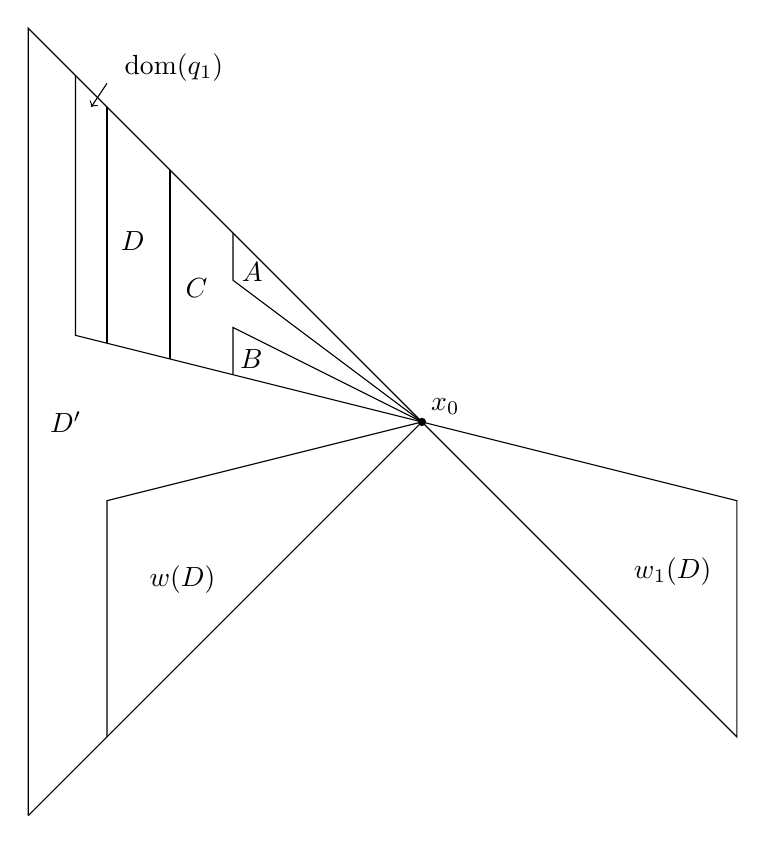
\begin{tikzpicture}[scale=0.1]

\draw (0,0) to (50,50) to (0,100) to (0,0);
\draw (10,10) to (10,40) to (50,50) to (90,40) to (90,10) to (50,50);
\draw (6, 94) to (6,61) to (50,50);
\draw (10, 60) to (10,90);
\draw (18, 58) to (18,82);
\draw (26, 56) to (26,62) to (50,50);
\draw (26, 74) to (26, 68) to (50,50);
\draw[->] (10,93) to (8,90);
\filldraw[fill=black, very thick] (50,50) circle (0.3);

\node[left] at (8, 50) {$D'$};
\node[left] at (25,30) {$w(D)$};
\node[left] at (88, 31) {$w_1(D)$};
\node[left] at (16, 73) {$D$};
\node[left] at (24, 67) {$C$};
\node[left] at (31, 69) {$A$};
\node[left] at (31, 58) {$B$};
\node[left] at (26,95) {$\mbox{dom}(q_1)$};
\node[left] at (56,52) {$x_0$};


\end{tikzpicture}
\caption{The composition of $D_1'$. \label{fig:1}}
\end{figure}
      
Extend the ordering on $D'$ to $D_1'$ so that the following hold:
    \begin{enumerate}
       \item[(a)] for any $y_1,y_2 \in D$, $w_1(y_1) < w_1(y_2)$ if and only if $w(y_1) < w(y_2)$;
       \item[(b)] for any $u \in A \cup B$ and $y \in D$, if $w(y) < b_n=\max(A\cup B)$, then $u<w_1(y)$ if and only if $u<w(y)$;
       \item[(c)] for any $y \in D$, if $w(y) > b_n$, then $a_n < w_1(y) <b_n$. 
    \end{enumerate}
    Such an extension clearly exists. 

Now define $g_1\colon A\cup w(D)\to A\cup w_1(D)$ by letting $g_1(a) = a$ for all $a\in A$ and $g_1(w(y)) = w_1(y)$ for all $y\in D$. Then $g_1$ is order-preserving by the above requirements (a) through (c). To see that $g_1$ is a partial isometry, let $a \in A$ and $y\in D$. Since $\mbox{dom}(q_1)\cup w(D)$ is the free amalgam of $\mbox{dom}(q_1)$ and $w(D)$ over $\{x_0\}$ and $D_1'$ is the free amalgam of $D'$ and $w_1(D)$ over $\{x_0\}$, we have \[d(a, w(y))=d(a,x_0)+d(x_0,w(y))=d(a,x_0)+d(x_0,w_1(y))=d(a,w_1(y)).\] 
    Intuitively, $g_1$ sends $w(y)$ to a copy which is smaller than $b_n$ and fixes $A$ pointwise. Consequently, we have $w_1(D)<b_n$ and, for any $y \in D$, $w_1(y) <x_0$ if and only if $w(y)<x_0$.
    
Let $w_2(D)$ be a fresh isomorphic copy of $w(D)$ such that $w_2(D)$ and $w(D)$ has exactly one common point $x_0$. Let $D_2'$ be the free amalgam of $D_1'$ and $w_2(D)$ over $\{x_0\}$. Extend the ordering on $D_1'$ to $D_2'$ so that the following hold:
 \begin{enumerate}
       \item[(d)] for any $y_1,y_2 \in D$, $w_2(y_1) < w_2(y_2)$ if and only if $w_1(y_1) < w_1(y_2)$;
       \item[(e)] for any $u \in A \cup B$ and $y \in D$, if $w(y) < a_n$, then $u<w_2(y)$ if and only if $u<w_1(y)$;
       \item[(f)] for any $y \in D$, if $w(y) > a_n$, then $b_{n-1} < w_2(y) <a_n$. 
    \end{enumerate}
Define an order-preserving partial isometry $g_2\colon B\cup w_1(D)\to B\cup w_2(D)$ by letting $g_2(b)=b$ for all $b\in B$ and $g_2(w_1(y))=w_2(y)$ for all $y\in D$. Moreover, $w_2(D) < a_n$ and, for any $y \in D$, $w_2(y) <x_0$ if and only if $w_1(y)<x_0$.
    
Repeating this construction, we obtain, for $1\leq i \leq 2n$, $D_i'=D' \cup w_1(D) \cup \dots \cup w_i(D)$, which can be viewed as the free amalgam of $w_i(D)$ and the remaining part over $\{x_0\}$, an ordering on $D_{2n}'$ extending that on $D'$, and order-preserving partial isometries $g_1, g_2, g_3, \dots,g_{2n}$ such that 
\begin{enumerate}
\item[(i)] for any $1\leq i\leq n$, $g_{2i-1}(a)=a$ for all $a\in A$, and $g_{2i}(b)=b$ for all $b\in B$;
\item[(ii)] for any $1\leq i\leq n$ and $y\in D$, $g_{2i}(w_{2i-1}(y))=w_{2i}(y)$, and $g_{2i-1}(w_{2i-2}(y))=w_{2i-1}(y)$ if $i>1$.
\end{enumerate}
Moreover, we have $w_{2n}(D) <a_1$ and, for any $y \in D$, $w_{2n}(y) <x_0$ if and only if $w(y)<x_0$. 

Define a map $$r\colon A\cup w_{2n}(C)\to A\cup w_{2n}(p(C))$$ by letting $r(a)=a$ for all $a\in A$ and $r(w_{2n}(c))=w_{2n}(p(c))$ for all $c\in C$. Then for $a \in A$ and $c \in C$,  we have
    \begin{align*}
    d(a,w_{2n}(c)) &=d(a,x_0)+d(x_0,w_{2n}(c))=d(a,x_0)+d(x_0,w(c))\\&=d(a,x_0)+d(x_0,c)=d(a,x_0)+d(x_0,p(c))\\&=d(a,x_0)+d(x_0,w(p(c))) \\
& =d(a,x_0)+d(x_0,w_{2n}(p(c)))=d(a,w_{2n}(p(c))) \\
&=d(r(a),r(w_{2n}(c))).
    \end{align*} 
Thus $r$ is a partial isometry. Note that $w$ and $p$ are order-preserving and each fixes $x_0$. Thus for any $c\in C$, we have 
    \begin{align*}
      w_{2n}(c)<x_0 &\iff w(c)<x_0 \iff c<x_0 \\&\iff p(c) <x_0 \iff w(p(c))<x_0 \\&\iff w_{2n}(p(c))<x_0. 
    \end{align*}
    Since for all $y \in D$, $w_{2n}(y)<a_1$, we conclude that $r$ is an order-preserving partial isometry. 



By Lemma~\ref{lemma:Extensions} and our construction, the distances in $D_{2n}'$ are all taken from the additive semigroup generated by the distances in $D$. Now redefine the metric on $D_{2n}'$ by taking the minimum of the original distance value and $\sup\Delta$. Call the resulting metric space $D''$. Since $D$ is a $\Delta$-metric space, it follows that $D''$ is a $\Delta$-metric space, and, as an ordered metric space, $D''$ is an extension of $D$. Moreover, each of the order-preserving partial isometries $q_1, q_2, g_1, g_2, \dots, g_{2n}, r$ continues to be order-preserving partial isometries of $D''$. 

Now by the weak homogeneity of $\mathbb{U}_{\Delta}^<$, we can extend $D$ to an isomorphic copy of $D''$ as a substructure of $\mathbb{U}_\Delta^<$. By the ultrahomogeneity of $\mathbb{U}_\Delta^<$, we can extend all the above order-preserving partial isometries to full automorphisms of $\mathbb{U}_{\Delta}^<$. Denote the resulting automorphisms by the same notation. Then for $1\leq i\leq 2n$, we have $r, q_1,g_i \in {\rm Aut}_A(\mathbb{U}_{\Delta}^<)$ if $i$ is odd, and $q_2,g_i \in {\rm Aut}_B(\mathbb{U}_{\Delta}^<)$ if $i$ is even. Finally, for any $c \in C$, \[p(c)=w(q_1,q_2)^{-1}g_1^{-1}\dots g_{2n}^{-1}rg_{2n}\dots g_1w(q_1,q_2)(c).\]
Thus if we let 
$$q=w(q_1,q_2)^{-1}g_1^{-1}\dots g_{2n}^{-1}rg_{2n}\dots g_1w(q_1,q_2), $$
then $q\in \langle {\rm Aut}_A(\mathbb{U}_\Delta^<), {\rm Aut}_B(\mathbb{U}_\Delta^<) \rangle$ and $p\upharpoonright C=q\upharpoonright C$ as required.
     \end{proof}

     \begin{lemma}\label{theorem:density}
        Let $\Delta$ be a countable distance value set, and let $A,B \subseteq \mathbb{U}_{\Delta}^<$ be finite subsets. Suppose $A \cap B = \varnothing$. Then \[\langle {\rm Aut}_A(\mathbb{U}_{\Delta}^<), {\rm Aut}_B(\mathbb{U}_{\Delta}^<) \rangle  \ is \ dense \ in \  {\rm Aut}(\mathbb{U}_{\Delta}^<).\]
\end{lemma}    

\begin{proof}   Let $p \in {\rm Aut}(\mathbb{U}_{\Delta}^<)$ and let $C \subseteq \mathbb{U}_{\Delta}^<$ be a finite subset. We show that there is a $q \in \langle {\rm Aut}_A(\mathbb{U}_{\Delta}^<), {\rm Aut}_B(\mathbb{U}_{\Delta}^<) \rangle$ such that $p\upharpoonright C=q\upharpoonright C$. Again we may assume $A\cup B \subseteq C$. Consider the ordered $\Delta$-metric space $C \cup p(C)$. Extend it to an ordered $\Delta$-metric space $C \cup p(C) \cup \{x_0\}$, where the metric is defined by 
$$d(x_0,y)=\mbox{diam}(C\cup p(C))=\max\{d(y_1,y_2)\colon y_1,y_2 \in C \cup p(C)\}$$
for any $y\in C\cup p(C)$, and the ordering is defined by $x_0 <y$ for all $y\in C\cup p(C)$.
           Such an extension can be found in $\mathbb{U}_{\Delta}^<$ by the weak homogeneity of $\mathbb{U}^<_\Delta$, and so we may assume $x_0 \in \mathbb{U}_{\Delta}^<$. Now consider $A' = A \cup \{x_0\}$, $B' = B \cup \{x_0\}$ and let $p' \in {\rm Aut}_{x_0}(\mathbb{U}_\Delta^<)$ be an extention of $p\upharpoonright C \cup \{(x_0,x_0)\}$. Applying Lemma~\ref{lemma:density} to $A', B'$ and $p'$, we get a $q \in \langle {\rm Aut}_{A'}(\mathbb{U}_{\Delta}^<), {\rm Aut}_{B'}(\mathbb{U}_{\Delta}^<) \rangle$ such that $q\upharpoonright C\cup\{x_0\}=p'\upharpoonright C\cup\{x_0\}$. Then in particular $q \in \langle {\rm Aut}_A(\mathbb{U}_{\Delta}^<), {\rm Aut}_B(\mathbb{U}_{\Delta}^<) \rangle$ and $q\upharpoonright C=p\upharpoonright C$ as required. 
        \end{proof}
 
We also need the following two lemmas about proper open subgroups of $\mbox{\rm Aut}(\mathbb{U}^<_\Delta)$.    

     \begin{lemma}\label{lemma:f_orbit}
        Let $V$ be a proper open subgroup of ${\rm Aut}(\mathbb{U}_{\Delta}^<)$. Then there exists an element $x \in \mathbb{U}_{\Delta}^<$ such that $V\cdot x$ is finite.
        \begin{proof}
           Toward a contradiction, assume $V\cdot x$ is infinite for all $x\in \mathbb{U}_{\Delta}^<$. We prove that $V$ is dense. Since $V$ is also closed, it follows that $V = {\rm Aut}(\mathbb{U}_{\Delta}^<)$, contradicting the properness of $V$. 

Note that a basic open neighborhood of the identity element of $\mbox{\rm Aut}(\mathbb{U}^<_\Delta)$ has the form ${\rm Aut}_{A}(\mathbb{U}_{\Delta}^<)$, where $A$ is a finite subset of $\mathbb{U}^<_\Delta$. Since $V$ is an open subgroup, there is a finite $A\subseteq \mathbb{U}^<_\Delta$ such that ${\rm Aut}_{A}(\mathbb{U}_{\Delta}^<) \subseteq V$. By Neumann's lemma (see Corollary 4.2.2 of Hodges \cite{Hodges}), there exists $g \in V$ such that $g(A)\cap A = \varnothing$. 
           
By Lemma~\ref{theorem:density}, $\langle {\rm Aut}_{A}(\mathbb{U}_{\Delta}^<), {\rm Aut}_{g(A)}(\mathbb{U}_{\Delta}^<) \rangle$ is dense in ${\rm Aut}(\mathbb{U}_{\Delta}^<)$. This group is contained in $V$, and thus $V$ is dense. 
        \end{proof}
     \end{lemma}

     %We use the following lemma to reconstruct $\mathbb{U}_\Delta^<$. 
     \begin{lemma}\label{lem:maxopen}
        Let $V$ be a proper open subgroup of ${\rm Aut}(\mathbb{U}_{\Delta}^<)$. The following are equivalent:
        \begin{enumerate}
           \item[\rm (1)] There exists a unique $x \in \mathbb{U}_{\Delta}^<$ such that $V = {\rm Aut}_{\{x\}}(\mathbb{U}_{\Delta}^<)$. 
           \item[\rm (2)] $V$ is maximal among proper closed subgroups of ${\rm Aut}(\mathbb{U}_{\Delta}^<)$. 
        \end{enumerate}
        \end{lemma}
\begin{proof}
           First suppose $V = {\rm Aut}_{\{x\}}(\mathbb{U}_{\Delta}^<)$. Assume $H$ is a closed subgroup of $\mbox{\rm Aut}(\mathbb{U}^<_\Delta)$ such that $V\subsetneq H\subsetneq \mbox{\rm Aut}(\mathbb{U}^<_\Delta)$.  Let $g \in H \setminus V$. Then $g(x) \neq x$ and ${\rm Aut}_{\{g(x)\}}(\mathbb{U}_{\Delta}^<) = g{\rm Aut}_{\{x\}}(\mathbb{U}_{\Delta}^<)g^{-1}=gVg^{-1} \leq H$. By Lemma~\ref{theorem:density}, $\langle {\rm Aut}_{\{g(x)\}}(\mathbb{U}_{\Delta}^<), {\rm Aut}_{\{x\}}(\mathbb{U}_{\Delta}^<) \rangle$ is dense in ${\rm Aut}(\mathbb{U}_{\Delta}^<)$. Since it is a subgroup of $H$ and $H$ is closed, we have $H= {\rm Aut}(\mathbb{U}_{\Delta}^<)$, contradicting the properness of $H$. 
     
           For the converse, assume (2) holds. By Lemma~\ref{lemma:f_orbit}, there exists an element $x \in \mathbb{U}_{\Delta}^<$ such that $V\cdot x$ is finite. We show that $V\subseteq \mbox{\rm Aut}_{\{x\}}(\mathbb{U}^<_\Delta)$. Otherwise, let $g \in V$ be such that $g(x) \neq x$. Then either $g(x)>x$ or $g(x)<x$. Since $g$ is order-preserving, we get that either $g^{n+1}(x) > g^n(x)$ for all natural numbers $n$, or $g^{n+1}(x)<g^n(x)$ for all natural numbers $n$. In either case, $V\cdot x$ is infinite. 
           
It is clear that $\mbox{\rm Aut}_{\{x\}}(\mathbb{U}^<_\Delta)\neq \mbox{\rm Aut}(\mathbb{U}^<_\Delta)$. Thus by the the maximality of $V$, we have
$V=\mbox{\rm Aut}_{\{x\}}(\mathbb{U}^<_\Delta)$.
     
           For the uniqueness, assume ${\rm Aut}_{\{x\}}(\mathbb{U}_{\Delta}^<) = {\rm Aut}_{\{y\}}(\mathbb{U}_{\Delta}^<)$ but $x \neq y$. Then by Lemma~\ref{theorem:density}, $\langle {\rm Aut}_{\{x\}}(\mathbb{U}_{\Delta}^<), {\rm Aut}_{\{y\}}(\mathbb{U}_{\Delta}^<) \rangle$ is dense. But $$\langle {\rm Aut}_{\{x\}}(\mathbb{U}_{\Delta}^<), {\rm Aut}_{\{y\}}(\mathbb{U}_{\Delta}^<) \rangle={\rm Aut}_{\{x\}}(\mathbb{U}_{\Delta}^<) = {\rm Aut}_{\{y\}}(\mathbb{U}_{\Delta}^<),$$ and thus they are both the whole group, which is impossible. 
        \end{proof}

     We are now ready to finish the proof of Theorem~\ref{thm:class}. Recall that the remaining direction is (i) implying (ii).

        Let $f\colon \mbox{\rm Aut}(\mathbb{U}^<_\Delta)\to\mbox{\rm Aut}(\mathbb{U}^<_\Lambda)$ be a topological group isomorphism. By Lemma~\ref{lem:maxopen}, for each $x \in \mathbb{U}_{\Delta}^<$, there is a unique $y \in \mathbb{U}_{\Lambda}^<$ such that $f({\rm Aut}_{\{x\}}(\mathbb{U}_{\Delta}^<))={\rm Aut}_{\{y\}}(\mathbb{U}_{\Lambda}^<)$. We write $y=g(x)$. The map $g$ is well-defined and bijective. 

        Note that for any $x,y,x',y'\in\mathbb{U}_{\Delta}^<$, ${\rm Aut}_{\{x,y\}}(\mathbb{U}_{\Delta}^<)$ and ${\rm Aut}_{\{x',y'\}}(\mathbb{U}_{\Delta}^<)$ are conjugate in $\mbox{\rm Aut}(\mathbb{U}^<_\Delta)$ if and only if $d(x,y)=d(x',y')$. Also note that
$$ {\rm Aut}_{\{x,y\}}(\mathbb{U}_{\Delta}^<)=\mbox{\rm Aut}_{\{x\}}(\mathbb{U}^<_\Delta)\cap \mbox{\rm Aut}_{\{y\}}(\mathbb{U}^<_\Delta) $$
and similarly for $\mbox{\rm Aut}_{\{x',y'\}}(\mathbb{U}^<_\Delta)$. Thus by the definition of $g$, we have that for any $x,y,x',y' \in \mathbb{U}_{\Delta}^<$,
$$ d(x,y)=d(x',y') \iff d(g(x),g(y)) = d(g(x'),g(y')).$$
        
Now for any $d \in \Delta$, we define $\theta(d) \in \Lambda$ by finding $x,y \in \mathbb{U}_{\Delta}^<$ such that $d(x,y)=d$, and then setting $\theta(d)=d(g(x),g(y))$. By the above observation, $\theta$ is well-defined and bijective. We show that $\theta$ witnesses the equivalence of $\Delta $ and $ \Lambda$. Suppose $(d_1,d_2,d_3)$ is a $\Delta$-triangle. There exist $x,y,z \in \mathbb{U}_{\Delta}^<$ such that the distances among them are exactly $(d_1,d_2,d_3)$. Then the distaces among $g(x),g(y),g(z)$ are $(\theta(d_1),\theta(d_2),\theta(d_3))$. Thus $(\theta(d_1),\theta(d_2),\theta(d_3))$ is a $\Lambda$-triangle. The converse also holds.

The proof of Theorem~\ref{thm:class} is complete.

\begin{thebibliography}{99}
\bibitem{EGLMM}
M. Etedadialiabadi, S. Gao, F. Le Ma\^{\i}tre, and J. Melleray,
\textit{Dense locally finite subgroups of automorphism groups of ultraextensive spaces},
Adv. Math. {\bf 391} (2021), 107966.

\bibitem{Hodges}
W. Hodges, 
Model Theory. Encyclopedia of Mathematics and its Applications,vol. 42.
 Cambridge University Press, Cambridge, 1993.

\bibitem{KPT}
A. S. Kechris, V. G. Pestov, and S. Tordocevic,
\textit{Fra\"{\i}ss\'{e} limits, Ramsey theory, and topological dynamics of automorphism groups},
Geom. Funct. Anal. {\bf 15} (2005), no. 1, 106--189.

\bibitem{Slutsky}
K. Slutsky,
\textit{Non-genericity phenomena in ordered Fra\"iss\'e classes},
J. Symb. Log. {\bf 77} (2012), no. 3, 987--1000.
\end{thebibliography}
\end{document}
